% CS669: Pattern Recognition
% Programming Assignment II
% Gabriel Dulac-Arnold <gabe@squirrelsoup.net>
% Johannes H. Jensen <johannj@stud.ntnu.no>
\documentclass[a4paper]{article}
\usepackage{multicol}
\usepackage{graphicx}
\usepackage[top=2cm,nohead,nofoot]{geometry}

\author{Gabriel Dulac-Arnold $<$gabe@squirrelsoup.net$>$ (CS09F004) \\
Johannes H. Jensen $<$johannj@stud.ntnu.no$>$ (CS09F005) \\
\\
(Batch no. 14)}
\title{CS669 - Pattern Recognition\\
\emph{Programming Assignment III}}

\begin{document}
\setlength{\parskip}{2ex}
\setlength{\tabcolsep}{8pt}
\renewcommand\arraystretch{1.5}
\maketitle

\section{Dataset I: Linearly Separable}

These are the linearly seperable datasets that allow us to visualize the basic functioning of the various linear classifiers.
All the classifiers perform well on these datasets except for one outlying point that consistently gets misclassified.

\subsection{Classifier Accuracy}

\begin{tabular}{ | l | r | }
\hline
\textbf{Classifier} & \textbf{Accuracy} \\
\hline
Fisher Discriminant  &   99.73\% \\
\hline
Perceptron          &   99.73\% \\
\hline
SVM                 &   ZERO\%   \\
\hline
\end{tabular}


\subsection{Confusion Matrices}

\begin{multicols}{2}
\begin{enumerate}
\item Fisher Discriminant:

\begin{tabular}{ | l | c | c | c | }
\hline
& $\omega_1$ & $\omega_2$ & $\omega_3$ \\
\hline
  $\omega_1$ & 124 & 1 & 0 \\
\hline
  $\omega_2$ & 0 & 125 & 0 \\
\hline
  $\omega_3$ & 0 & 0 & 125 \\
\hline
\end{tabular}

\item Batch Perceptron:

\begin{tabular}{ | l | c | c | c | }
\hline
& $\omega_1$ & $\omega_2$ & $\omega_3$ \\
\hline
  $\omega_1$ & 124 & 0 & 1 \\
\hline
  $\omega_2$ & 0 & 125 & 0 \\
\hline
  $\omega_3$ & 0 & 0 & 125 \\
\hline
\end{tabular}
\columnbreak

\item SVM:

\begin{tabular}{ | l | c | c | c | }
\hline
& $\omega_1$ & $\omega_2$ & $\omega_3$ \\
\hline
  $\omega_1$ & NOPE & 0 & 1 \\
\hline
  $\omega_2$ & 0 & NEIN & 0 \\
\hline
  $\omega_3$ & 0 & 0 & NIET \\
\hline
\end{tabular}
\end{enumerate}
\end{multicols}


\newpage
\subsection{Decision Region Plots}

\begin{figure}[htbp!]
\center
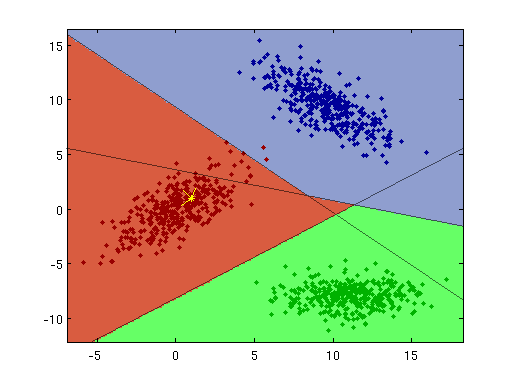
\includegraphics[clip, trim=40px 15px 30px 10px]{ls_fisher.png}
\caption{Fisher Discriminant}
\end{figure}



\newpage
\section{Dataset II: Overlapping Data}
Fisher Discriminant does a good job of finding pertinent boundaries, but the overlapping nature of the dataset makes classification difficult.
\subsection{Classifier Accuracy}

\begin{tabular}{ | l | r | }
\hline
\textbf{Classifier} & \textbf{Accuracy} \\
\hline
Fisher Discriminant  &   89.6\% \\
\hline
SVM          &   OUU\% \\
\hline

\end{tabular}

\subsection{Confusion Matrices}

\begin{multicols}{2}
\begin{enumerate}
\item Fisher Discriminant:

\begin{tabular}{ | l | c | c | c | }
\hline
& $\omega_1$ & $\omega_2$ & $\omega_3$ \\
\hline
  $\omega_1$ & 108 & 16 & 1 \\
\hline
  $\omega_2$ & 2 & 116 & 7 \\
\hline
  $\omega_3$ & 10 & 3 & 112 \\
\hline
\end{tabular}

\item SVM:

\begin{tabular}{ | l | c | c | c | }
\hline
& $\omega_1$ & $\omega_2$ & $\omega_3$ \\
\hline
  $\omega_1$ & NOT & 16 & 1 \\
\hline
  $\omega_2$ & 2 & TRUE & 7 \\
\hline
  $\omega_3$ & 10 & 3 & ATALL \\
\hline
\end{tabular}

\end{enumerate}
\end{multicols}

\subsection{Decision Region Plots}

\begin{figure}[htbp!]
\center
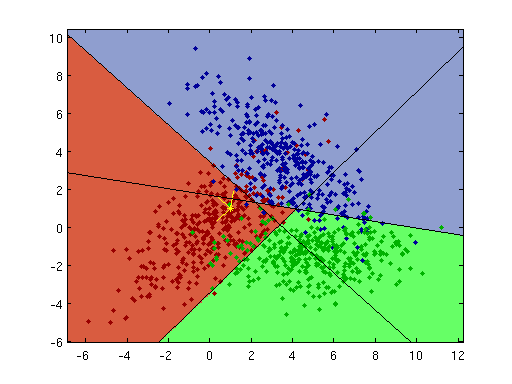
\includegraphics[clip, trim=40px 15px 30px 10px]{nls_fisher.png}
\caption{Fisher Discriminant}
\end{figure}

\section{Dataset III: Real World Image Feature Data}

\subsection{Classifier Accuracy}

\begin{tabular}{ | l | r | }
\hline
\textbf{Classifier} & \textbf{Accuracy} \\
\hline
Bayes Single Gaussian  &   58.67\% \\
\hline
Bayes PCA Gaussian  &   60.00\% \\
\hline
Fisher Discriminant  &   70.67\% \\
\hline
SVM          &   ou\% \\
\hline
\end{tabular}


\subsection{Confusion Matrices}

\begin{multicols}{2}
\begin{enumerate}

\item Bayes Single Gaussian:

\begin{tabular}{ | l | c | c | c | }
\hline
& $\omega_1$ & $\omega_2$ & $\omega_3$ \\
\hline
  $\omega_1$ & 20 & 1 & 4 \\
\hline
  $\omega_2$ & 10 & 7 & 8 \\
\hline
  $\omega_3$ & 5 & 3 & 17 \\
\hline
\end{tabular}

\item Bayes PCA Gaussian:

\begin{tabular}{ | l | c | c | c | }
\hline
& $\omega_1$ & $\omega_2$ & $\omega_3$ \\
\hline
  $\omega_1$ & 9 & 2 & 14 \\
\hline
  $\omega_2$ & 0 & 18 & 7 \\
\hline
  $\omega_3$ & 3 & 4 & 18 \\
\hline
\end{tabular}
\columnbreak
\item Fisher Discriminant:

\begin{tabular}{ | l | c | c | c | }
\hline
& $\omega_1$ & $\omega_2$ & $\omega_3$ \\
\hline
  $\omega_1$ & 16 & 2 & 7 \\
\hline
  $\omega_2$ & 3 & 20 & 2 \\
\hline
  $\omega_3$ & 1 & 7 & 17 \\
\hline
\end{tabular}

\end{enumerate}
\end{multicols}


\section{Conclusions}

In this assignement we see the performance of linear classifiers with gradually more complex datasets.  We don't use explicitly non-linear datasets as these would of course not work well with these techniques, but we do realize that for real-world high-dimensional applications, linear classifiers and dimensional reduction techniques work much better than Gaussian Bayes classifiers.

\end{document}

